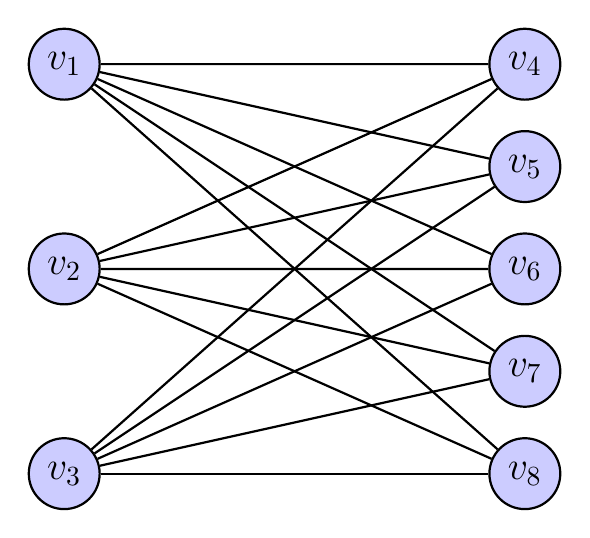
\begin{tikzpicture}[
  scale=1.3,
  vnode/.style={circle, fill=blue!20, draw=black, thick, minimum size=9mm, inner sep=0pt, font=\Large}
]
  % Partición izquierda
  \node[vnode] (v1) at (0, 4) {$v_1$};
  \node[vnode] (v2) at (0, 2) {$v_2$};
  \node[vnode] (v3) at (0, 0) {$v_3$};

  % Partición derecha
  \foreach \j in {4,...,8} {
    \node[vnode] (v\j) at (4.5, {8-\j}) {$v_{\j}$};
  }

  % Aristas: cada vértice de la izquierda con cada vértice de la derecha
  \foreach \i in {1,2,3} {
    \foreach \j in {4,...,8} {
      \draw[thick] (v\i) -- (v\j);
    }
  }
\end{tikzpicture}
